\chapter {MOTION SYNTHESIS FRAMEWORK}
\label{chap:msf}
\graphicspath{{CombineFramework/CombineFrameworkFigs/EPS/}{CombineFramework/CombineFrameworkFigs/}}
The principal ideas of \moit are discussed in previous two chapters.
Stability of motion is controlled by maintaining the topology, 
for periodic motion, neural oscillator can be used to enhance the structural stability.
And group Transformation provides a mechanism to modify motion with precision.


Questions rise when these ideas are being applied  to \cms.
The first question comes from idea combination.

The ideas of Global Motor Invariant and Local Motor Invariant are dicussed separately in Chapter~\ref{chap:gi} and Chapter~\ref{chap:li}.
This chapter focuses on put these ideas into \cms application.
Two problems arised from combinations in application
\begin{itemize}
	\item Combine global and local motor invariant controller together.
	\item Combine different motion primitives together.
\end{itemize}

\section{Combined Motor Invariant Control}

\subsection{ Combine Motor Invariant Control}

Neural Oscillator will maintain the Global Motor Invariant and Controlled Symmetry will maintain the Local Motor Invariant.
Combining two controllers poses the question of violating the other invariant:
\begin{itemize}
\item From the Global Motor Invariant Perspective in Chapter~\ref{chap:gi},
when the controlled symmetry  is applied, it must not violate the topology. 
It is easy to prove that controlled symmetry maintains the topology.

\item From the Local Motor Invariant perspective in Chapter~\ref{chap:li}.
Controlled symmetry can only applied to mechanical system, the \cpg will not be effected by controlled symmetry.
When a group action is applied to the mechanical system, parameters of \cpg should be transformed accordingly to maintain the symmetry property.
This is called \emph{Adjoint Transformation}.
\end{itemize}


In application, to ajust the combined controller,
\cpg is applied first maintain the topology against the structural perturbation. 
Afterwards Symmetry Control is to meet application specific constraints.
This idea is illustrated in the following Figure ~\ref{fig:sysoverview}

\begin{figure}[!htbp]
  \begin{center}
      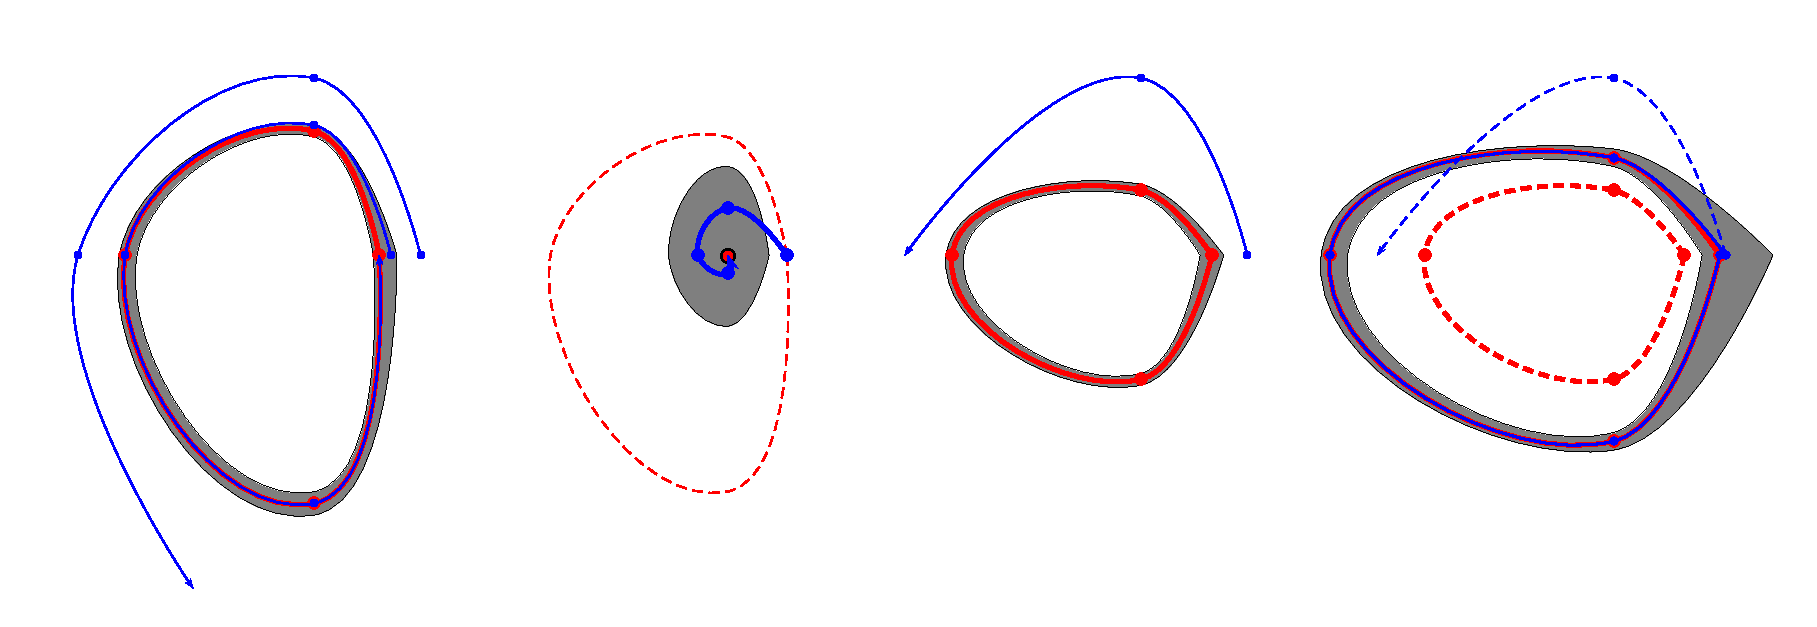
\includegraphics[width=0.7\textwidth]{LimitCircle}
    \caption{System Over View }
    \label{fig:sysoverview}
  \end{center}
\end{figure}


For the controlled symmetry's effect on topology, we have the following theorem:

\begin{mythe}
Transformation of Control Symmetry is Topological Conjugation
\end{mythe}
\begin{proof}
This theorem is easy to prove by checking properties of group.
\end{proof}

\subsection{Adjoint Transformation of \cpg}
Adjoint Transformation modify the parameters of neural oscillator to maintain the symmetry.

Coupled with neural oscillator, the dynamic system 
\[
\dot{\state}=F(\state)
\]
becomes a system 
\begin{equation}
\label{eq:gc}
\dot{\state}=F(\state)+D\uout
\end{equation}


When the symmetry group action $g$ is applied, the Equations~\ref{{eq:gc}} are transformed into
\begin{equation}
\label{eq:cc}
Tg(\dot{\state})=F(g(\state))+DTg(\uout)
\end{equation}




If symmetry is preserved, the Equation~\ref{eq:con} and Equation~\ref{eq:cc} should be equivalent.
\begin{equation}
\label{eq:con}
\dot{\state}=F(\state)+\ulocal+D\tilde{\uout}
\end{equation}
$\tilde{\uout}$ is the output of neural ssytem after adjoint transformation.
As show in equation~\ref{eq:simplematsuta},$\uout$ is a function of $\uin$.
Control effort can not be directly on neural oscillator, transformation of $\uout$ is achieved by modifying the system's parameters.



\begin{myprop}
By modifying parameter $\tau_{1,2}$
\[
\tau_{1,2} \mapsto \ep \tau_{1,2}
\]
is equivalent to time scaling the neural oscillator by parameter $\ep$.
\end{myprop}
\begin{proof}
By subsitute $\tilde{\tau}_{1,2}=\ep \tau_{1,2}$, and $\tilde{t}=\frac{t}{\ep}$, the Equation~\ref{eq:matsuta} will remain the same.
\end{proof}

Based on the propostion above, a scheme of adjoint transformation to modify the parameters $\tau_{1,2}$,$\hin$,$\hout$ for maintain the symmetry of the  coupled system.
The input and output of neural are chosen to maintain the shape.
\begin{enumerate}
\item Modify $\tau$ by the time scaling parameter $\tau \mapsto \ep \tau$.
\item Input variable $w$ and input efficient $\hin$ are modified to make sure the input function statisfy the time scaling symmetry $\uin(t) \mapsto \uin(\frac{t}{\ep})$
\item  Parameters of $\hout$ are modified according to $D$, or how the mechanical system is drived.
If $\uout$ drive the position variable $q$ then, $\hout$ should multiplied by the position scale factor. 
If $\uout$ drive the velocity,$\hout$ is multiplied by the speed scale factor.
If the $hout$ is force and acting on the acceleration $\ddot{q}$, then $\hout$ is multiplied by the acceleration scale facotr.
\end{enumerate}


According this adjoint transformation strategy, we can get the following thereom
\begin{mythe}
For a transformation group $G$, if the parameters of the neural oscillator are modified according to adjoint transformation.
 Combined system preserving symmetry $I^G$.
\end{mythe}
For prove, readers can check the symmetry by substitute transformed variables into the original system to check the symmetry.

Thus both the Local Motor Invariant and Global Motor Invariant are maintained
For the specific symmetry types proposed in Chapter~\ref{chap:li},several example of adjoint symmetry are provideds


\subsubsection*{ Offset Symmetry.}
For offset symmetry:
\[
(t,q,\qd) \mapsto (t,q+\ep,\qd)
\]
there is no time scaling effects.
To maintain the shape of $\uin$ and $\uout$,  $\uin$ and $\uout$ are functions in invariant space.
For example, the input of the neural oscillator are chosen to be the angle difference between the joints or velocity.



\subsubsection*{Time Scaling}
For time scaling:
\[
(t,q,\qd) \mapsto (\frac{t}{\ep},q,\ep \qd)
\]
Adjoint Transformation
$\tau \mapsto \ep \tau $.
if the output$\uout$ is applied as force, then $\hout \mapsto \ep^2 \hout$

\subsubsection*{ Energy Scaling}
Energy Scaling is combined action of time scaling and posture scaling:
\[
(t,q,\qd ) \mapsto ( \frac{f(\ep)}{\ep}t ,f(\ep)q,\ep\qd)
\]
the time scalling factor is $\frac{\ep}{f(\ep)}$, 

The parameters $\tau_{1,2}$ are transformed
\[
\tau_{1,2} \mapsto \frac{\ep}{f(\ep)} \tau_{1,2}
\]
To maintain the time scaling symmetry of $\uin$, if the input valuable is $\qd$, 
then 
\[
\hin \mapsto \ep \hin
\]
if the output drive the velocity, then the output is $\hout$
\[
\hout \mapsto \ep \hout
\]




\subsection{Example: Height Control of Bouncing Ball}

Bouncing Ball has energy scaling symmetry; a limit cycle emerged when coupling with neural oscillator.
By combining both motor invariant controllers, the limit cycle can be controlled.
Then the bouncing height can be controlled.

\subsubsection*{Adjoint Transformation}
Suppose the coupled system is bouncing at height of $5$
For the energy scaling:
\[
(t,q,\qd ) \mapsto ( \ep t ,\ep^2 q,\ep \qd)
\]

According to the system transformation
the time scaling factor is $\ep$, we have:
\[
\tau_{1,2} \mapsto \alpha \tau_{1,2}
\]

The input to the neural oscillator is $\qd$,
\[
\hin \mapsto \frac{\hin}{\ep}
\]
 
Neural Oscillator drives the position of the paddle, the output $\uout$ needs to be scaled by the position scale value.
For $q \mapsto \ep^2q$, we have
\[
 \hout \mapsto \ep^2 \hout
\]

When $\ep^2=3$, then the ball will bounce at height of $15$, and it maintain its topological structure, which is a limit cycle.
as shown in Figure ~\ref{fig:energy3}. 
By this method, arbitrary bouncing height can be controlled.


\begin{figure}[!htbp]
  \begin{center}
   	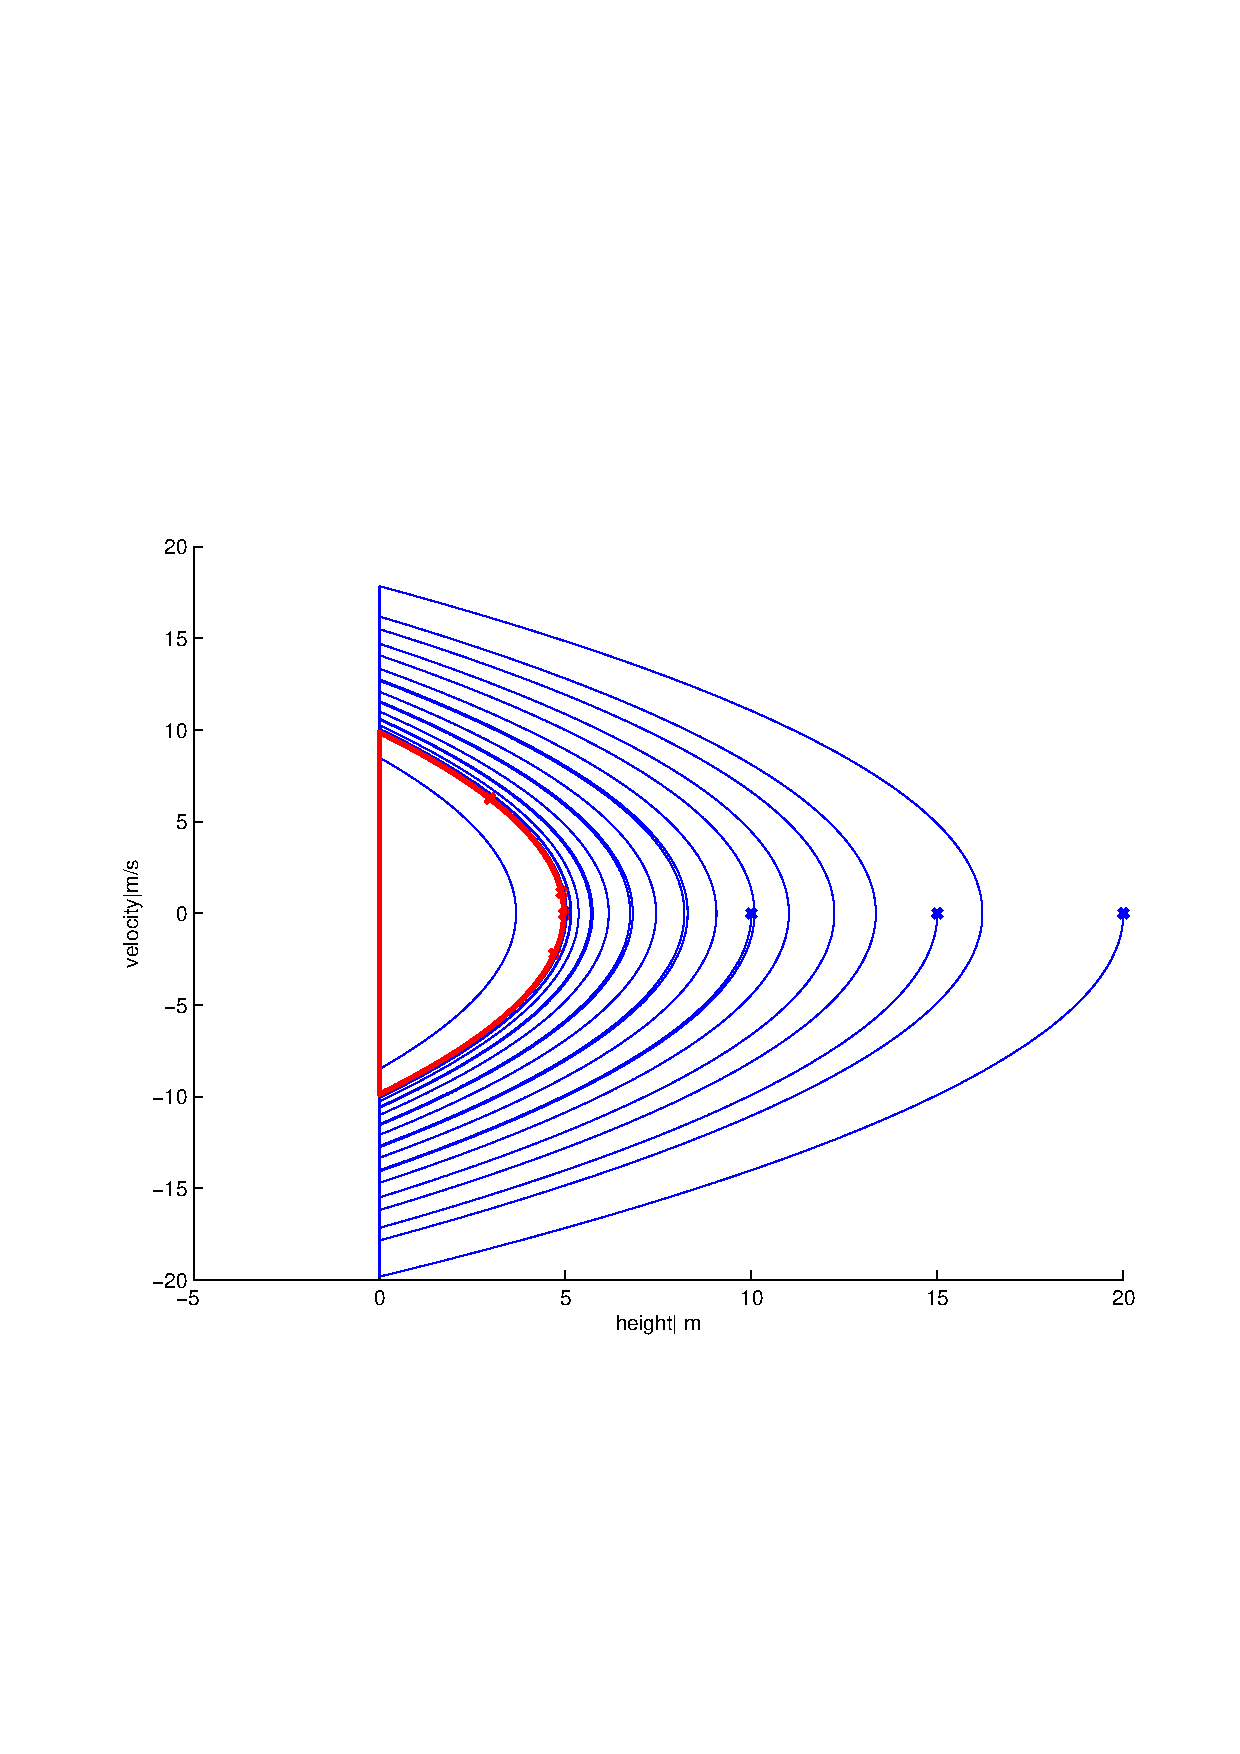
\includegraphics[width=0.7\textwidth]{BouncingBallPhasePlotAction1}
    \caption{Energy Scalling}
    \label{fig:energy1}
  \end{center}
\end{figure} 


\begin{figure}[!htbp]
  \begin{center}
	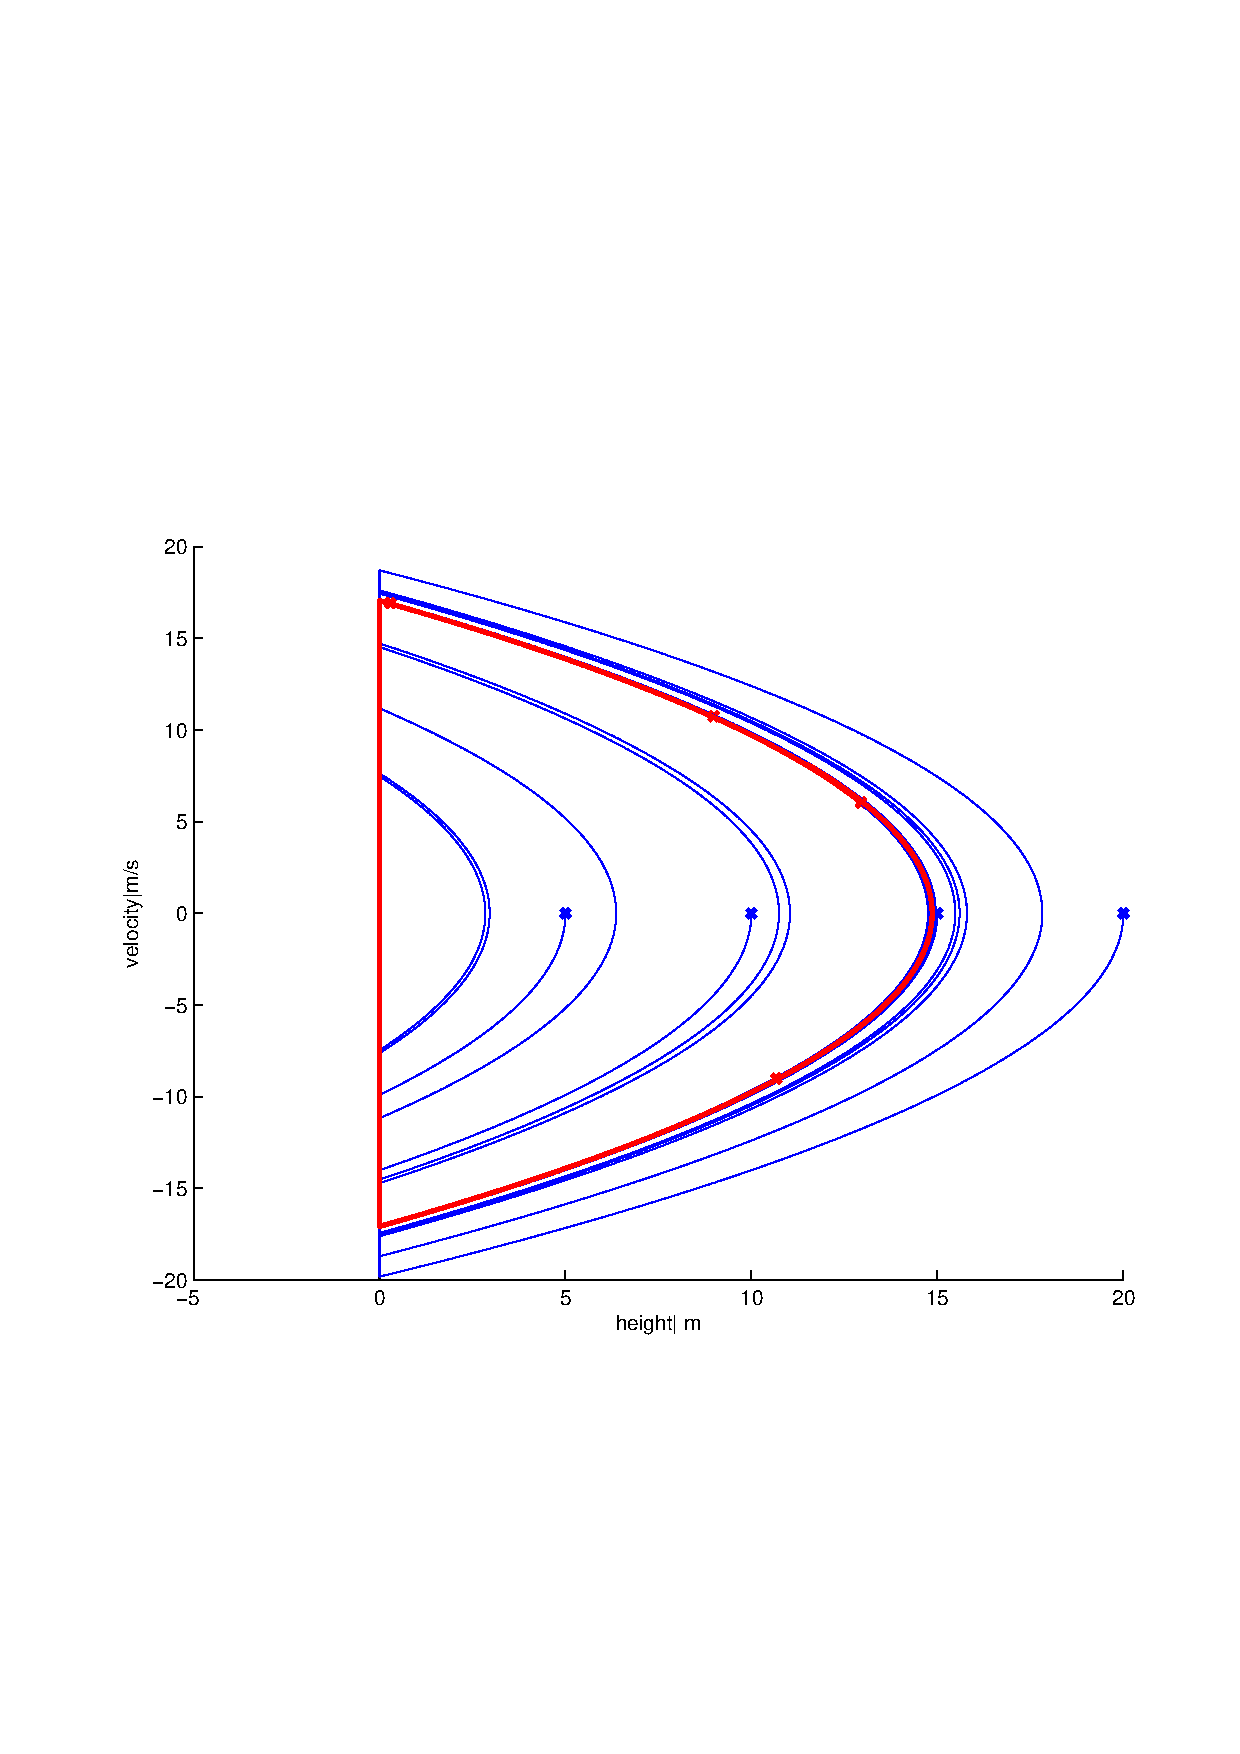
\includegraphics[width=0.7\textwidth]{BouncingBallPhasePlotAction3}
    \caption{Energy Scaling}
    \label{fig:energy3}
  \end{center}
\end{figure}

\section{Combine Motion Primitives}

\subsection{Dynamic Motion Graph}
The topological structure of the natural mechanical syste form a graph structure:
Each motion primitive is represented as a node, and two nodes are conneced if they are near each other on the phase plot.
This graph is the \emph{Dynamic Motion Graph}.

The idea is very similar to the \emph{Motion Graph}\citep{kovar2008motion}, the difference is in the  Motion Graph are handed crafted.
While in our research,  the dynamic motion graph is fixed, from any motion primitive, the motion primitive a character can changed to is limited.

\begin{figure}[!htbp]
  \begin{center}
	\includegraphics[width=0.7\textwidth]{MotionPrimitiveGraph}
    \caption{Phase Plot of Motion Primitives}
    \label{fig:manyprimitives}
  \end{center}
\end{figure}


\begin{figure}[!htbp]
  \begin{center}
      \includegraphics[width=0.7\textwidth]{motiongraphtopology}
    \caption{Phase Plot of Motion Primitives}
    \label{fig:manyprimitives}
  \end{center}
\end{figure}


\subsection{Dynamic Motion Primitives Transition}
From  the dynamic perspective, motion primitive transition means move the current $\state$ from the basin of attraction of one attractor into another, as shown in Figure~\ref{fig:motion-transition}.
Without any effort, the transition will not happen automatically, for the two basic of attractions do not overlap.



\begin{figure}[!htbp]
  \begin{center}
      \includegraphics[width=0.7\textwidth]{MotionPrimitiveTransition}
    \caption{Motion Primitive Transition}
    \label{fig:motion-transition}
  \end{center}
\end{figure}


Based on the two methods for motor invariant control, two methods are proposed for motion primitive transition.
\begin{itemize}
\HiItem{Entrainment Overlap}
Empirically,when \cpg is applied for one motor primitive $\mathcal{A}$, the basin of attraction $\mathcal{Bo}(\mathcal{A})$ is enlarged.
If \cpg are applied for two motion primtives $\mathcal{A,A'}$ seperately, the enlarged basin of attractions $\mathcal{Bo}(\mathcal{A})$,
%$\omicron$
$\mathcal{Bo}(\mathcal{A'})$ will overlap.
\[
O =
\mathcal{Bo}(\mathcal{A}) 
\bigcap \mathcal{Bo}(\mathcal{A'}) 
\neq \varnothing
\]
 
If  state $\state$ lies in the $O$, by switch the \cpg controller, motion primitive is also switched, as shown in Figure~\ref{fig:motion-overlay}.


\begin{figure}[!htbp]
  \begin{center}
      \includegraphics[width=0.7\textwidth]{OverLayTransition}
    \caption{OverLay Transition}
    \label{fig:motion-overlay}
  \end{center}
\end{figure}


\HiItem{Transform Method}
Controlled Symmetry can also apply for motion primitive transition.
For a system at $\state$,  The phase portrait can be transformed to move the basin of attraction,as shown in Figure~\ref{fig:transform-offset}.


\begin{figure}[!htbp]
  \begin{center}
      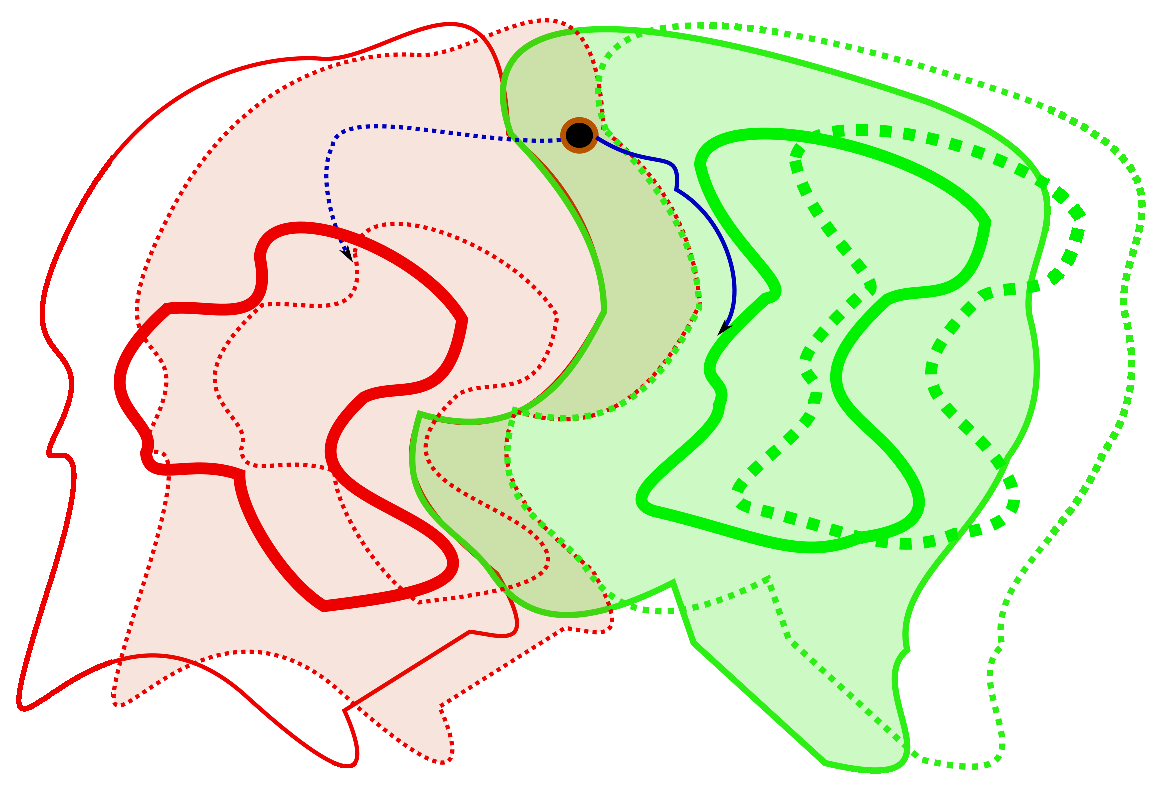
\includegraphics[width=0.7\textwidth]{OffsetTransition}
    \caption{Offset Transiton}
    \label{fig:transform-offset}
  \end{center}
\end{figure}
\end{itemize}




Both the method can result in physically realistic motion transition, but requires $\state$ lies at specific reason.
In motor invariant theory, the current state $\state$ is not directly controlled.
The measure is make the overlap region $O$ cover part of both attractors$\mathcal{A}$,$\mathcal{A'}$.

The state $\state$ is going to converge to the attractor $\mathcal{A}$.
The overlap region cover both attractors $\mathcal{A}$, $\mathcal{A'}$,bidirectional transitions are possible when motions are near stable state.

When Controlled Symmetry is applied, both motion primitives are transformed, there is relationship between the two transformations; \emph{transformation connection}, as shown in Figure~\ref{fig:Combine}

\begin{figure}[!htbp]
  \begin{center}
      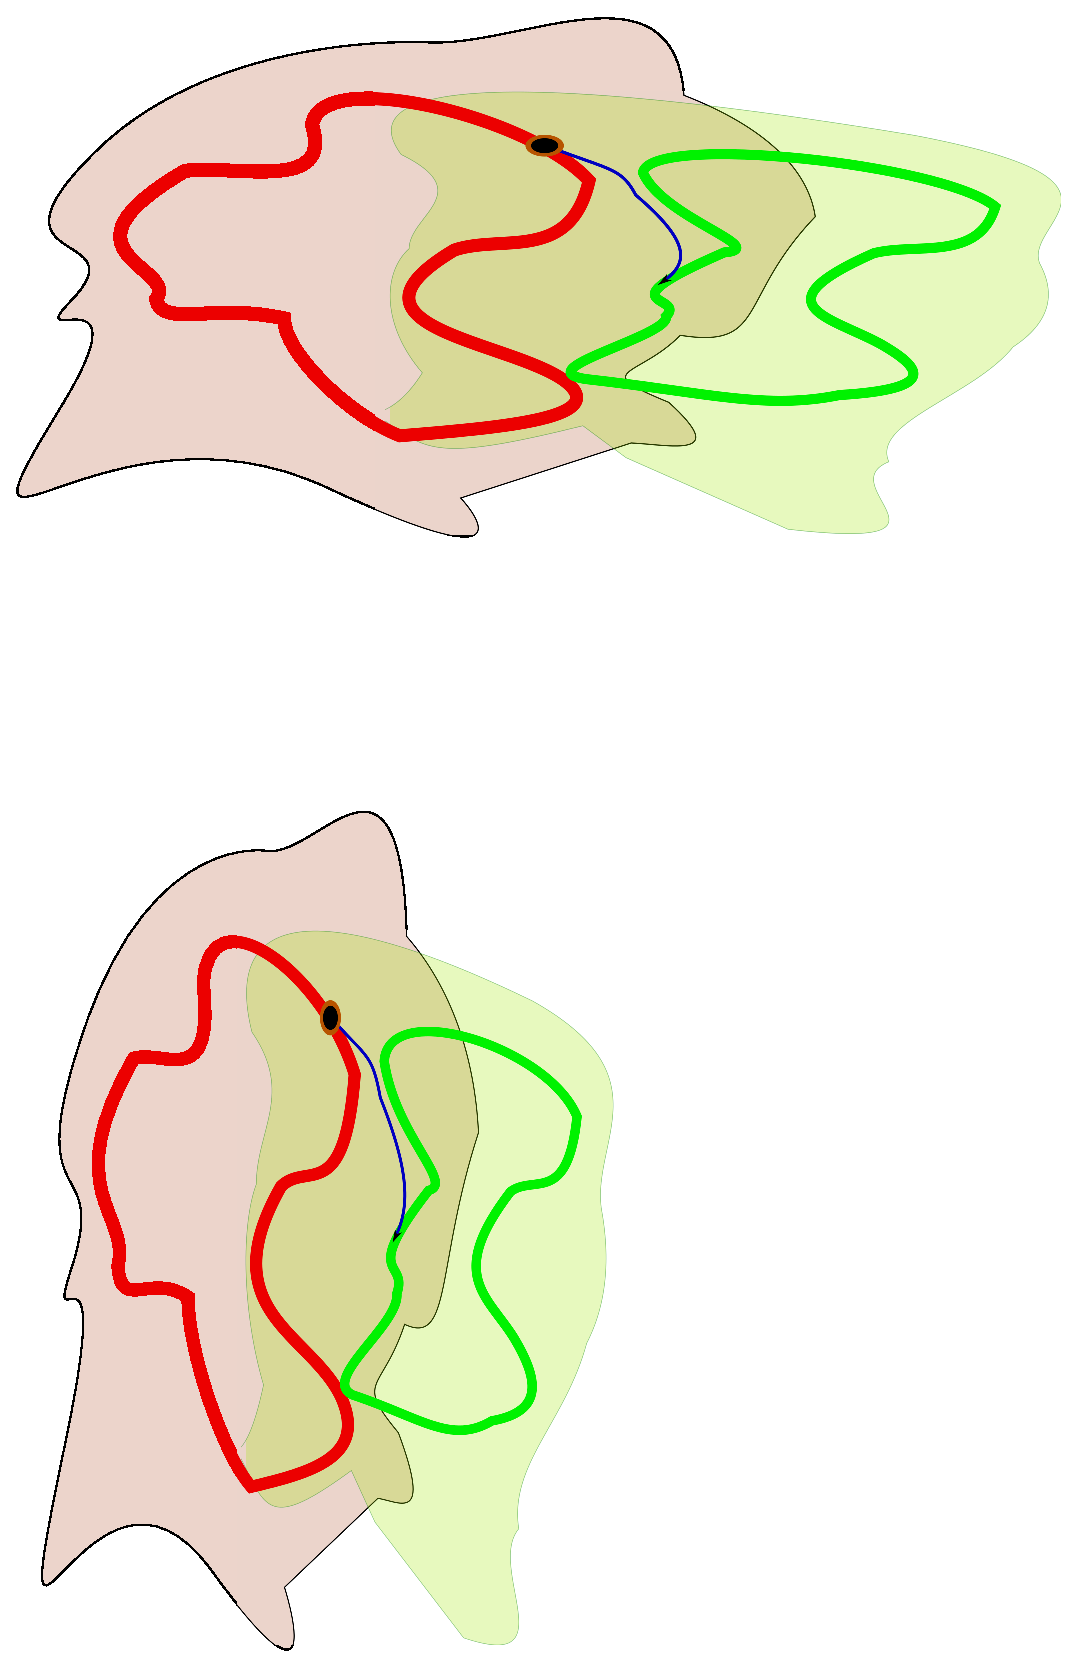
\includegraphics[width=0.7\textwidth]{ConbineMethod}
    \caption{Comined Method}
    \label{fig:Combine}
  \end{center}
\end{figure}

\section{Motion Synthesis Framework}
While this procedure may appear mathematically complex, applying this method for motion synthesis is straightforward. 
You will need:
\begin{enumerate}
\item a mechanical oscillator $F(\x)$ which best describes the body and environment
\item a neural oscillator (for example, the Matsuoka oscillator in Equation~\ref{eq:matsuta}) and associated parameters,that form a limit cycle

\item an action $g \in G$ which adapts the problem to the current environment (we present three possible operators in Section~\ref{sec:control_symmetry}). the adjoint system transformation  is applied to the neural oscillator parameters.

\item an integrator to solve the system (we use the fourth order Runge--Kutta method provided in the {MATLAB} function \emph{ode45}).
\end{enumerate}
In the following chapters, this method is applied to generationg adaptive motions.



